% Note: Ensure \usepackage{tikz}, \usetikzlibrary{positioning}, and \usepackage{pgfplots} are included in your main preamble.

\chapter{Mutual Information Neural Estimation (MINE)}
\label{ch:mine}

\section{The Challenge of Measuring Dependence in High Dimensions}

% 1. Descriptive opening
Information theory provides an exceptionally powerful lens through which to view representations in deep learning. As discussed in previous chapters, quantities such as the mutual information $I(X; Z)$ between input data $X$ and latent representations $Z$ can illuminate the dynamics of learning, the compression of nuisance factors, and the sufficiency of learned features. The Information Bottleneck principle, for instance, formulates the goal of representation learning entirely in terms of mutual information: maximizing $I(Z; Y)$ while minimizing $I(X; Z)$. However, estimating these mutual information terms in the context of modern neural networks presents a formidable theoretical and computational challenge.

Mutual information is fundamentally a measure of dependence between random variables. When the variables in question are low-dimensional and discrete, estimating $I(X; Z)$ is a straightforward matter of counting empirical frequencies to approximate the joint and marginal distributions. When the variables are continuous and one-dimensional, techniques such as kernel density estimation (KDE) or simple histogram binning provide reliable approximations. But in deep learning, $X$ often represents high-dimensional data such as high-resolution images, complex audio waveforms, or dense text embeddings. Similarly, the latent representation $Z$ typically resides in spaces spanning hundreds or thousands of dimensions. In these high-dimensional regimes, traditional non-parametric density estimation fails catastrophically due to the curse of dimensionality. The number of samples required to reliably estimate the joint probability density function scales exponentially with the number of dimensions. With a finite dataset $\mathcal{D}$, the empirical density estimates become impossibly sparse and variance-dominated.

Furthermore, because we only have access to empirical samples from the joint distribution---namely, our dataset and the deterministic or stochastic mappings induced by our neural networks---we cannot compute $I(X; Z)$ by explicitly integrating over analytical probability densities. For many years, this intractability forced researchers to rely on restrictive parametric assumptions. One common assumption is that all distributions involved are multivariate Gaussians, which reduces mutual information to a function of covariance matrices. Alternatively, researchers used crude variational bounds that were analytically tractable but often too loose to be practically useful in high dimensions, fundamentally limiting our ability to measure and optimize true information-theoretic quantities during training.

The paradigm shifted significantly with the introduction of Mutual Information Neural Estimation (MINE). Rather than attempting the impossible task of explicitly estimating high-dimensional probability densities, MINE reframes the estimation of mutual information as a continuous optimization problem over a family of functions parameterized by a neural network. By leveraging classical variational representations of the Kullback-Leibler (KL) divergence, MINE constructs a lower bound on the mutual information that can be maximized using standard stochastic gradient descent. The neural network, which we will denote as $f_\theta$, acts as a highly expressive "critic" or discriminator. Its sole purpose is to learn to distinguish between samples drawn from the true joint distribution (where variables are dependent) and samples drawn from the product of the marginal distributions (where variables are independent).

This approach elegantly bridges information theory and deep learning. It allows us to estimate mutual information in arbitrarily high-dimensional, continuous settings by relying on the very same computational workhorse that created the representations in the first place: the neural network itself. By framing estimation as optimization, MINE allows us to scale mutual information estimation to modern deep learning architectures and massive datasets.

In this chapter, we develop the rigorous mathematical foundations of MINE. We will prove the variational bounds that make it possible, beginning with the Donsker-Varadhan representation. We will analyze the statistical properties of the resulting estimators, examining the subtle challenges of biased gradients that arise when implementing these estimators with stochastic minibatches. Finally, we will compare the Donsker-Varadhan bound with alternative $f$-divergence representations, equipping you with the theoretical tools needed to apply MINE to real-world representation learning problems.

\section{The Mathematical Foundations of MINE}

% 2. Mathematical core
We begin by recalling the definition of mutual information in terms of the Kullback-Leibler divergence. For two random variables $X$ and $Z$ defined over spaces $\mathcal{X}$ and $\mathcal{Z}$, with joint distribution $\mathbb{P}_{XZ}$ and marginal distributions $\mathbb{P}_X$ and $\mathbb{P}_Z$, the mutual information is exactly the KL divergence from the product of the marginals to the joint distribution:
\begin{equation}
    I(X; Z) = D_{\text{KL}}(\mathbb{P}_{XZ} \parallel \mathbb{P}_X \otimes \mathbb{P}_Z).
\end{equation}
The core mathematical engine of MINE is the Donsker-Varadhan representation of the KL divergence, which expresses $D_{\text{KL}}$ as a supremum over a space of bounded measurable functions. By optimizing over this function space, we can estimate the divergence without ever estimating the underlying densities.

\subsection{The Donsker-Varadhan Representation}

\begin{theorem}[Donsker-Varadhan Representation]
\label{thm:dv}
Let $\mathbb{P}$ and $\mathbb{Q}$ be two probability measures on a measurable space $\Omega$. The Kullback-Leibler divergence admits the following variational representation:
\begin{equation}
    D_{\text{KL}}(\mathbb{P} \parallel \mathbb{Q}) = \sup_{T: \Omega \to \mathbb{R}} \left( \mathbb{E}_{\mathbb{P}}[T(\omega)] - \log \mathbb{E}_{\mathbb{Q}}[e^{T(\omega)}] \right),
\end{equation}
where the supremum is taken over all functions $T$ such that the two expectations are finite.
\end{theorem}

\begin{proof}
Let $T: \Omega \to \mathbb{R}$ be any measurable function satisfying the integrability conditions. We construct a new probability measure $\mathbb{G}$, often called the Gibbs measure, defined by its Radon-Nikodym derivative with respect to $\mathbb{Q}$:
\begin{equation}
    d\mathbb{G}(\omega) = \frac{e^{T(\omega)}}{Z} d\mathbb{Q}(\omega), \quad \text{where the partition function is } Z = \mathbb{E}_{\mathbb{Q}}[e^{T(\omega)}].
\end{equation}
Because $\mathbb{G}$ is a valid probability measure, the fundamental property of the KL divergence ensures that $D_{\text{KL}}(\mathbb{P} \parallel \mathbb{G}) \geq 0$. We can expand this divergence:
\begin{align}
    0 \leq D_{\text{KL}}(\mathbb{P} \parallel \mathbb{G}) &= \mathbb{E}_{\mathbb{P}} \left[ \log \frac{d\mathbb{P}}{d\mathbb{G}} \right] \\
    &= \mathbb{E}_{\mathbb{P}} \left[ \log \left( \frac{d\mathbb{P}}{d\mathbb{Q}} \frac{d\mathbb{Q}}{d\mathbb{G}} \right) \right] \\
    &= \mathbb{E}_{\mathbb{P}} \left[ \log \frac{d\mathbb{P}}{d\mathbb{Q}} \right] + \mathbb{E}_{\mathbb{P}} \left[ \log \left( Z e^{-T(\omega)} \right) \right].
\end{align}
Recognizing the first term as $D_{\text{KL}}(\mathbb{P} \parallel \mathbb{Q})$, we can distribute the expectation in the second term:
\begin{equation}
    0 \leq D_{\text{KL}}(\mathbb{P} \parallel \mathbb{Q}) - \mathbb{E}_{\mathbb{P}}[T(\omega)] + \log Z.
\end{equation}
Substituting $Z = \mathbb{E}_{\mathbb{Q}}[e^{T(\omega)}]$ and rearranging the terms yields the lower bound:
\begin{equation}
    D_{\text{KL}}(\mathbb{P} \parallel \mathbb{Q}) \geq \mathbb{E}_{\mathbb{P}}[T(\omega)] - \log \mathbb{E}_{\mathbb{Q}}[e^{T(\omega)}].
\end{equation}
To show that the supremum is achievable (and thus the bound is tight), we consider the optimal function $T^*(\omega) = \log \frac{d\mathbb{P}}{d\mathbb{Q}}(\omega)$. Substituting $T^*$ into our bound gives:
\begin{align}
    \mathbb{E}_{\mathbb{P}}[T^*(\omega)] - \log \mathbb{E}_{\mathbb{Q}}[e^{T^*(\omega)}] &= \mathbb{E}_{\mathbb{P}}\left[ \log \frac{d\mathbb{P}}{d\mathbb{Q}}(\omega) \right] - \log \mathbb{E}_{\mathbb{Q}}\left[ \frac{d\mathbb{P}}{d\mathbb{Q}}(\omega) \right] \\
    &= D_{\text{KL}}(\mathbb{P} \parallel \mathbb{Q}) - \log (1) \\
    &= D_{\text{KL}}(\mathbb{P} \parallel \mathbb{Q}).
\end{align}
Since $\mathbb{E}_{\mathbb{Q}}[\frac{d\mathbb{P}}{d\mathbb{Q}}] = \int d\mathbb{P} = 1$, the logarithm vanishes. Thus, the bound is tight, and the supremum is attained exactly when the function $T(\omega)$ equals the log-density ratio.
\end{proof}

\subsection{The MINE Estimator and the Critic Network}

By applying Theorem \ref{thm:dv} to the estimation of mutual information, we identify $\mathbb{P}$ with the joint distribution $\mathbb{P}_{XZ}$ and $\mathbb{Q}$ with the product of marginals $\mathbb{P}_X \otimes \mathbb{P}_Z$. The optimal function would be $T^*(x,z) = \log \frac{d\mathbb{P}_{XZ}}{d(\mathbb{P}_X \otimes \mathbb{P}_Z)}(x,z)$. 

Because searching over the space of all possible measurable functions is computationally intractable, MINE restricts the supremum to a rich family of functions parameterized by a neural network, $f_\theta: \mathcal{X} \times \mathcal{Z} \to \mathbb{R}$, with parameters $\theta \in \Theta$. This gives us the MINE objective:
\begin{equation}
\label{eq:mine_objective}
    I(X; Z) \geq I_{\Theta}(X; Z) \triangleq \sup_{\theta \in \Theta} \left( \mathbb{E}_{\mathbb{P}_{XZ}}[f_\theta(x,z)] - \log \mathbb{E}_{\mathbb{P}_X \otimes \mathbb{P}_Z}[e^{f_\theta(x,z)}] \right).
\end{equation}

The network $f_\theta$ acts as a critic. Its objective is to output high values for pairs $(x, z)$ sampled from the joint distribution (where $z$ is the actual representation of $x$) and low values for pairs sampled from the product of marginals (where a representation $z$ is randomly paired with an unrelated input $x'$). By the universal approximation theorem, as the capacity of the neural network $f_\theta$ increases, the parameterized bound $I_{\Theta}(X; Z)$ tightly approaches the true mutual information $I(X; Z)$.

In practice, we estimate this objective using minibatches. Given a batch of $N$ empirical samples $\{(x_i, z_i)\}_{i=1}^N \sim \mathbb{P}_{XZ}$, we synthesize samples from the product of marginals by simply dropping the joint association. This is elegantly achieved by shuffling the batch along the $z$ dimension to obtain $\{(x_i, z_{\pi(i)})\}_{i=1}^N \sim \mathbb{P}_X \otimes \mathbb{P}_Z$, where $\pi$ is a random permutation. The empirical MINE estimator is then defined as:
\begin{equation}
    \widehat{I}_{\text{MINE}}(\theta) = \frac{1}{N} \sum_{i=1}^N f_\theta(x_i, z_i) - \log \left( \frac{1}{N} \sum_{j=1}^N e^{f_\theta(x_j, z_{\pi(j)})} \right).
\end{equation}

\begin{figure}[htpb]
\centering
\begin{tikzpicture}[
    node distance=1.5cm and 2cm,
    box/.style={draw, rectangle, rounded corners, minimum width=2.5cm, minimum height=1cm, align=center, fill=blue!5},
    arrow/.style={-stealth, thick}
]

% Nodes
\node[box] (joint) {Joint Sample $(x, z) \sim \mathbb{P}_{XZ}$};
\node[box, below=of joint] (marginal) {Marginal Sample $(x, \tilde{z}) \sim \mathbb{P}_X \otimes \mathbb{P}_Z$};

\node[box, right=of joint, fill=red!5] (T1) {Critic $f_\theta$};
\node[box, right=of marginal, fill=red!5] (T2) {Critic $f_\theta$};

\node[right=of T1] (exp1) {$\mathbb{E}[f_\theta]$};
\node[right=of T2] (exp2) {$\log \mathbb{E}[e^{f_\theta}]$};

\node[box, right=1.5cm of exp1, yshift=-1.25cm, fill=green!5] (loss) {Maximize $\widehat{I}_{\text{MINE}}$};

% Arrows
\draw[arrow] (joint) -- (T1);
\draw[arrow] (marginal) -- (T2);
\draw[arrow] (T1) -- (exp1);
\draw[arrow] (T2) -- (exp2);

\draw[arrow] (exp1.east) -- (loss.north west);
\draw[arrow] (exp2.east) -- (loss.south west);

\end{tikzpicture}
\caption{Block diagram of the MINE architecture. The critic network $f_\theta$ processes samples from both the joint distribution (positive samples) and the product of marginal distributions (negative samples generated via permutation). The objective is maximized via backpropagation.}
\label{fig:mine_arch}
\end{figure}

\subsection{Gradient Bias and the $f$-Divergence Bound}

Maximizing the empirical estimator $\widehat{I}_{\text{MINE}}$ via stochastic gradient descent poses a subtle but significant statistical challenge. The exact gradient of the objective with respect to the network parameters $\theta$ is given by:
\begin{equation}
\label{eq:mine_grad}
    \nabla_\theta \widehat{I}_{\text{MINE}} = \mathbb{E}_{\mathbb{P}_{XZ}}[\nabla_\theta f_\theta(x,z)] - \frac{\mathbb{E}_{\mathbb{P}_X \otimes \mathbb{P}_Z}[\nabla_\theta f_\theta(x,z) e^{f_\theta(x,z)}]}{\mathbb{E}_{\mathbb{P}_X \otimes \mathbb{P}_Z}[e^{f_\theta(x,z)}]}.
\end{equation}
When we evaluate this gradient over minibatches during training, we substitute the expectations with their minibatch sample means. However, the expectation of a ratio is not equal to the ratio of expectations. Consequently, replacing the denominator with a minibatch average yields a \emph{biased} stochastic gradient. 

While increasing the batch size $N$ reduces this bias (it is asymptotically unbiased as $N \to \infty$), an elegant engineering solution is to use an exponential moving average to estimate the denominator across consecutive training steps. By smoothing the estimate of the denominator, we significantly reduce the bias without incurring the prohibitive memory cost of massive batch sizes.

Alternatively, researchers often turn to a different variational formulation based on $f$-divergences, specifically the Nguyen-Wainwright-Jordan (NWJ) bound. The NWJ bound avoids the logarithm of an expectation entirely:
\begin{equation}
    I(X; Z) \geq \sup_{\theta} \left( \mathbb{E}_{\mathbb{P}_{XZ}}[f_\theta(x,z)] - \mathbb{E}_{\mathbb{P}_X \otimes \mathbb{P}_Z}\left[e^{f_\theta(x,z) - 1}\right] \right).
\end{equation}
Because the logarithm is absent, this bound admits an strictly unbiased empirical gradient over minibatches. However, this comes at a theoretical cost: the NWJ bound is mathematically looser than the Donsker-Varadhan bound, often requiring larger function capacities or longer training to achieve the same estimation accuracy.

\subsection{Numerical Example: Correlated Gaussians}

To demonstrate the efficacy of MINE, let us examine a controlled synthetic environment. Consider a bivariate Gaussian distribution $(X, Z) \sim \mathcal{N}(0, \Sigma)$, where the covariance matrix is defined by a correlation coefficient $\rho \in (-1, 1)$:
\begin{equation}
    \Sigma = \begin{pmatrix} 1 & \rho \\ \rho & 1 \end{pmatrix}.
\end{equation}
Because both variables are standard normal, the true analytical mutual information is known exactly:
\begin{equation}
    I(X; Z) = -\frac{1}{2} \log (1 - \rho^2).
\end{equation}
By setting $\rho = 0.9$, the true mutual information is $I(X; Z) \approx 0.83$ nats. We can train a simple multi-layer perceptron (MLP) as our critic $f_\theta$ to maximize the MINE objective on samples drawn from this distribution. As the network trains, it gradually refines its continuous representation of the log-density ratio until the lower bound saturates near the analytical value.

\begin{figure}[htpb]
\centering
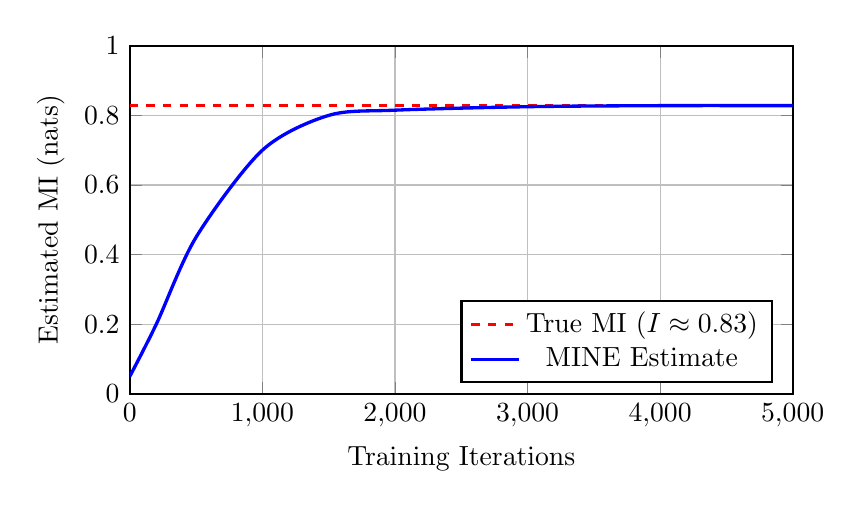
\begin{tikzpicture}
\begin{axis}[
    width=10cm,
    height=6cm,
    xlabel={Training Iterations},
    ylabel={Estimated MI (nats)},
    xmin=0, xmax=5000,
    ymin=0, ymax=1.0,
    grid=major,
    legend pos=south east,
    thick
]
% Analytical value line
\addplot[mark=none, color=red, dashed, very thick] coordinates {(0, 0.829) (5000, 0.829)};
\addlegendentry{True MI ($I \approx 0.83$)}

% Simulated MINE optimization curve
\addplot[mark=none, color=blue, very thick, smooth] coordinates {
    (0, 0.05) (200, 0.2) (500, 0.45) (1000, 0.70) (1500, 0.80) (2000, 0.815) (3000, 0.825) (4000, 0.828) (5000, 0.828)
};
\addlegendentry{MINE Estimate}
\end{axis}
\end{tikzpicture}
\caption{Optimization trajectory of MINE on a bivariate Gaussian with correlation $\rho = 0.9$. The estimated mutual information, bounded by the network capacity, closely asymptotes to the true analytical value of 0.83 nats as the critic network converges.}
\label{fig:mine_gaussian}
\end{figure}

The success of MINE in this highly controlled toy example scales impressively to higher dimensions, enabling empirical measurements for the Information Bottleneck principle and forming the backbone of contrastive representation learning techniques explored in subsequent chapters.

% 4. Summary + exercises
\section{Summary}

In this chapter, we introduced Mutual Information Neural Estimation (MINE), a technique that casts the estimation of mutual information as an optimization problem.
\begin{itemize}
    \item We derived the Donsker-Varadhan representation of the Kullback-Leibler divergence, mathematically proving that it acts as a tight lower bound for $D_{\text{KL}}(\mathbb{P} \parallel \mathbb{Q})$.
    \item We demonstrated how parameterizing the Donsker-Varadhan supremum with an expressive neural network allows us to estimate $I(X; Z)$ in high dimensions by merely discriminating between true joint samples and randomized marginal samples.
    \item We highlighted the issue of biased minibatched gradients that arise from the logarithm of an expectation, and introduced the alternative $f$-divergence (NWJ) bound as an unbiased but looser alternative.
\end{itemize}

\section*{Exercises}

\begin{enumerate}
    \item \textbf{Tightness of the $f$-Divergence Bound:} Prove the Nguyen-Wainwright-Jordan (NWJ) lower bound on KL divergence: $D_{\text{KL}}(\mathbb{P} \parallel \mathbb{Q}) \geq \sup_T \left( \mathbb{E}_{\mathbb{P}}[T] - \mathbb{E}_{\mathbb{Q}}[e^{T - 1}] \right)$. Find the optimal function $T^*$ that achieves equality, and compare it to the optimal function for the Donsker-Varadhan bound.
    \item \textbf{Gradient Bias Analysis:} Derive the gradient equation presented in Equation \ref{eq:mine_grad}. Prove mathematically why substituting the sample mean for $\mathbb{E}_{\mathbb{P}_X \otimes \mathbb{P}_Z}[e^{f_\theta}]$ inside the denominator results in a biased estimator for the gradient. Use Jensen's Inequality to determine the expected direction (sign) of this bias.
    \item \textbf{Empirical Implementation:} Implement MINE in PyTorch or TensorFlow to estimate the mutual information of a 10-dimensional multivariate Gaussian with a known covariance matrix. Compare the variance of your mutual information estimates during training using the DV bound versus the NWJ bound.
\end{enumerate}

% 3. Horizon box (Moved to the end per STYLE_GUIDE)
\begin{horizon}
While MINE represents a substantial theoretical and practical breakthrough in mutual information estimation, its scalability to arbitrarily high dimensions remains an active frontier. It is conjectured that in scenarios where $I(X; Z)$ is extremely large---such as deterministic autoencoders where the representation is a nearly lossless compression of the input---the Donsker-Varadhan bound suffers from catastrophic variance. Because the critic network $f_\theta$ must exponentiate its outputs for the marginal samples in the denominator, large target mutual informations require exponentially large outputs. This can easily induce numerical instability, gradient explosion, and unbounded variance in the estimator.

An open question is whether we can discover novel variational bounds that achieve variance reduction in these deterministic limits without sacrificing the tightness of the bound. Future work might show that regularizing the Lipschitz constant of the critic network via spectral normalization or gradient penalties could enforce smoothness constraints that reliably bound this variance, but whether this fundamentally limits the capacity of the network to estimate the true mutual information remains to be rigorously proven. Furthermore, it is conjectured that unifying MINE with optimal transport---for instance, using Wasserstein distances to smooth the manifold space prior to density estimation---could bypass the ratio-of-densities problem altogether, unlocking stable MI estimation for perfectly deterministic networks.
\end{horizon}

% TODO-CITE: Ensure all named results are cited.
